\documentclass[letterpaper,10 pt,conference]{ieeeconf}

\IEEEoverridecommandlockouts
\overrideIEEEmargins

\usepackage[utf8]{inputenc}
\usepackage[T1]{fontenc}

\usepackage{graphics} % for pdf, bitmapped graphics files
%\usepackage{mathptmx} % assumes new font selection scheme installed
\usepackage{times} % assumes new font selection scheme installed
\usepackage{amsmath} % assumes amsmath package installed
\usepackage{amssymb}  % assumes amsmath package installed
\usepackage[backend=bibtex8,style=ieee,sorting=none]{biblatex}

\usepackage{graphics} % for pdf, bitmapped graphics files
\usepackage{caption}
\usepackage{subcaption}
\usepackage{standalone}
\usepackage{tikz}
\usepackage{tikzscale}
\usetikzlibrary{calc}

\graphicspath{{img/}}
\addbibresource{references.bib}

\title{\LARGE \bf
  Optimizing Topometric Maps for Teach and Repeat
}


\author{David Landry and Alexandre Gari\'epy}


\begin{document}

\maketitle
\thispagestyle{empty}
\pagestyle{empty}


\begin{abstract} Topometric maps are a convenient approach to record reference points (also called
anchor points) in the Teach and Repeat paradigm. When using such a map, the question of how sparsely
the environment should be sampled arises. A very dense sampling will be more robust at the cost of
an increased database size. Fewer anchor points will make the use of loop-closure algorithms
easier. To replace the traditional approach of recording data at a regular intervals based on the
odometry of the wheels, we propose an offline algorithm that automatically filters the anchor points
points in a way that guarantees a certain tolerance to error. The topometric map then contains the
minimal amount of nodes required to execute the \textit{repeat} runs, making loop-closure easier and
allowing the mapping of longer trajectories. Offline experiments confirmed the ability of our
approach to optimize topometric maps, and showed that the size of the map will vary given a certain
demanded error tolerance.
\end{abstract}

\section{INTRODUCTION}

Teach and Repeat is a popular and efficient paradigm to execute tasks where it is possible to have
an operator show the robot how to execute it beforehand. It has been implemented using stereo
cameras \cite{Furgale10} or lidar sensors \cite{Sprunk13}. As shown in \cite{Furgale10}, an hybrid
between metric and topographic maps is an appropriate way to record a series of anchor points during
a \textit{teach} run. We will refer to those maps as \textit{topometric}. One of the questions that
arises when implementing such a navigation algorithm is how sparsely should the environement should
be mapped. A very frequent sampling, with lots of \textit{anchor points} to localize against during
the \textit{repeat} run, will provide more robustness to the algorithm. However the robustness comes
at the cost of a very large database size. The database size is in itself a burden but more
importantly if affects the performance of an eventual loop closure algorithms.

The current approach leaves it to the operator to decide how frequently an anchor point is
recorded. Both in \cite{Furgale10} and \cite{Sprunk13} the robot is told to record a new anchor
point at regular intervals, based on the odometry of the wheels. This approach comes with no
consideration for the complexity of the environment, and the operator has to guess what parameter
would be appropriate for a given application.

Inspired by \cite{Churchill15}, we will implement an algorithm such that there is no need for this
guesswork. By carefully evaluating ability of the anchor points to localize the robot on the taught
trajectory, we will be able to remove the unnecessary ones while still guaranteeing a certain
tolerance to error during the \textit{repeat} phase. Instead of choosing at what frequency the
environment is mapped, the operator will now have to wonder what tolerance to error he needs, which
is a more natural decision to make given a certain application.


\section{PROBLEM DEFINITION}

In our current implementation of the Teach and Repeat paradigm, the maps we use to repeat a
trajectory contains anchor points, transformations to go from one anchor to another, as well as
recorded commands for the whole trajectory. This paper, however, is focused on how to improve the
size of the underlying topometric map, without consideration for the list of commands.

We begin with an unoptimized topometric map, containing $N$ a set of interconnected nodes and $T$
the geometric transformations to go from one node to it's neighbor. The nodes in $N$ are in fact
anchor points to our teach an repeat implementation. They are point clouds in this case, but could
be any mean of localization, like the features of an image. Every node $n_i$ has an associated point
cloud $p_i$. The nodes are linked as a chain, from the first node recorded to the last.

Our objective is to find the smallest subset of $N$ such that the robot can reliably localize itself
against an anchor point at any time while it follows the taught trajectory. To decide wether the
robot can localize itself at a given position on the taught trajectory, we will induce an error in
the transformation estimate between both nodes. The intuition behind it is that by inducing
increasingly large errors, and having the ICP succeed nontheless, we can guarantee an increasingly
large robustness when going in the field. When the induced error becomes large enough, the
localisation will fail: the ICP algorithm converge in a local minimum, and the result of the ICP will
be largely different than the induced error.

\section{OUR APPROACH}
\label{approach}

\subsection{Deciding if a reading and anchor point pair can be used for localization}
\label{approach-deciding-converge}

First, lets define the terms reading and anchor point:

\begin{itemize}
  \item \textbf{Anchor point:} an anchor point is a node $n_i$ the nodes of the unoptimized
    topometric map. Each anchor point has an associated point cloud $p_i$. This point cloud is used
    as the reference point cloud when performing the ICP algorithm.
  \item \textbf{Reading:} a reading is the point cloud produced by the robot sensor during the
    repeat phase. However, we do the optimization of the topometric map in an offline process using
only the teach data. Therefore, we use simulated reading. To simulate a reading, we use the point
cloud $p_j$ of an anchor point and induce an error. This error is a 2D translation vector $[x,y]^T$, where $x$ is the forward-backword error and $y$ is the left-right error.
\end{itemize}

Lets consider a reading $r$ and an anchor point $a$. We know that $r$ is derived from inducing an error $[x, y]^T$ to $p_r$, which is associated to a node $n_r$.
We also know that the anchor point $a$ is associated to a node $n_a$ and a point cloud $p_a$. We can easily get the transform $t$ between $n_r$ and $n_a$ from $T$.


We want to know if $a$ can be used to localize $r$. To do so, we run the ICP algorithm using $r$ as the input and $p_a$ as the reference, using $t$
as the initialization of the ICP. ICP returns a transform $[x_{icp}, y_{icp}]^T$. We would except that ICP corrects the induced error by returning
a transformation $[-x, -y]^T$. This is verified by checking if the norm of the vector $[x_{icp}, y_{icp}]^T - [-x, -y]^T$ is under a certain $\epsilon$.


\subsection{Convergence ellipse}
Given two nodes $n_i$ and $n_j$ in $N$, we can use $n_j$ to generate readings and $n_i$ as an anchor
point.  We define the concept of a convergence ellipse as the ellipse around $n_i$ where we generate
readings by inducing error corresponding to the position in the ellipse, the center of the ellipse
being no induced error. We call the ellipse a convergence ellipse because each generated reading can
be used for localization using the $n_j$ anchor point, as described in the section
\ref{approach-deciding-converge} We chose the ellipse because it's shape corresponds to the motion
model of most ground robots. Throughout this paper, we define the ellipse by it's semiaxis $a$ and $b$.

Verifying if an ellipse is a convergence ellipse for a pair of nodes can be though of as fitting an
ellipse inside the convergence bassin seen in figure \ref{convergence_bassin}. This figure
represents, for a pair nodes $n_i$ and $n_j$, the size of the error after we ran the ICP with a
certain induced error. We also make the assumption that the bassin of convergence has a reasonable
shape and does not contain any holes. This assumption allows us to sample the function represented
on figure \ref{convergence_bassin} only on the edges of the ellipse, and make our algorithm much
more efficient. It also allows us to make a pretty sparse sampling of the edges of the ellipse: in
our experiment we sample 20 points around the ellipse and verify that the corresponding induced
error can still converge during ICP.

\begin{figure}[thpb]
  \centering
  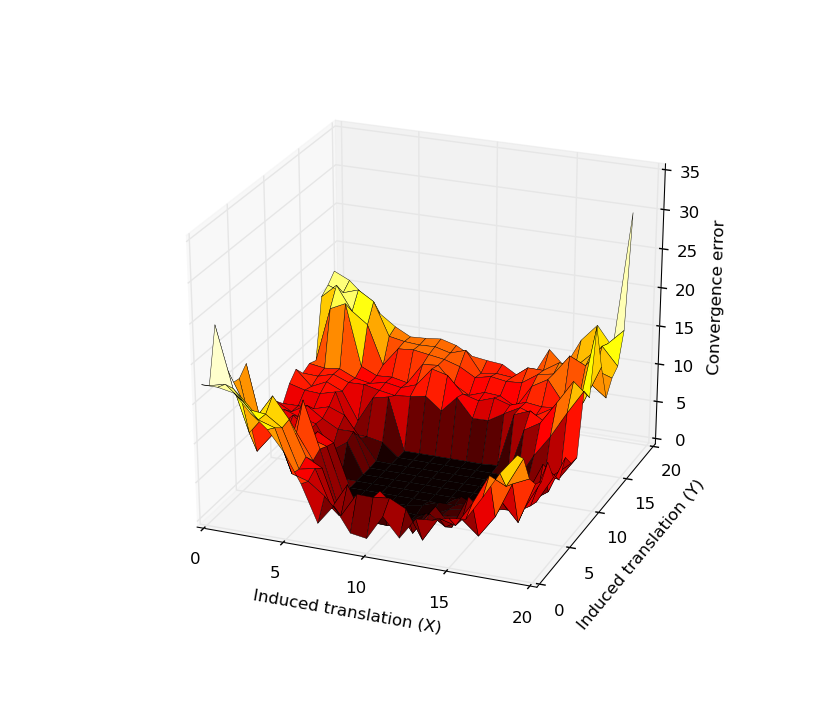
\includegraphics[scale=0.4]{convergence_bassin}
  \caption{The covergence bassin of a pair of readings}
  \label{convergence_bassin}
\end{figure}

\subsection{Mapping matching readings}
\label{matching-readings}
To reduce the size of the topometric map, we need to filter out nodes that are considered to add no
value to the map. To do so, we check how far appart can a reading and an anchor point be while still
be usable for localization. More formally, for each node $n_i$, we verify if an ellipse of readings
of a predetermined size is a convergence ellipse for the anchor point located at $n_{i+2}$,
$n_{i+3}$... $n_{i+k}$ until we find the node where the readings of the ellipse don't converge to
the anchor point $n_{i+k}$. We assume that the anchor point $n_{i+1}$ is always valid.

The results of this search are represented as an oriented graph, where an edge from $n_{i}$ to
$n_{j}$ means that the the ellipse of readings around $n_{j}$ is a convergence ellipse using the
node $n_i$ as the anchor point. An example graph is represented on figure \ref{graph_unoptimized}.

\begin{figure}[thpb]
  \centering
  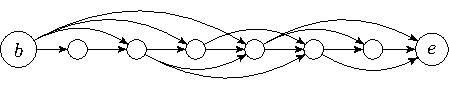
\includegraphics[scale=1.0]{unoptimized-graph}
  \caption{Representing convergence ellipses as an oriented graph}
  \label{graph_unoptimized}
\end{figure}


\subsection{Smallest topometric map}

To determine the smallest topometric map that still can be used for localization, we need to
eliminate redundant nodes.  For example, if the anchor point $n_{i+2}$ can be used for localization
of the readings around the node $n_i$, there is no need to keep the node $n_{i+1}$ in the map.

The graph reprensentation presented in the section \ref{matching-readings} allows to easily solve
this problem. If each edge on the graph has a cost of 1, the minimal topometric map from the
beginning of the map (node $b$) to the end of the map (node $e$) can be found using the Dijkstra's
algorithm \cite{dijkstra}. The nodes used on the shortest path from $b$ to $e$ are the minimal node
subset of the optimal topometric map. Note that the way the graph is built, it is guaranteed to be
acyclic, therefore Dijkstra's algorithm will always find the minimal node subset.


\begin{figure}[thpb]
  \centering
  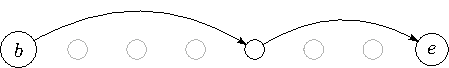
\includegraphics[scale=1.0]{optimized-graph}
  \caption{Optimal node subset using the graph approach and Dijkstra's algorithm}
\end{figure}


\section{EXPERIMENTS}

\subsection{Map optimization}

\begin{figure}
  \centering
  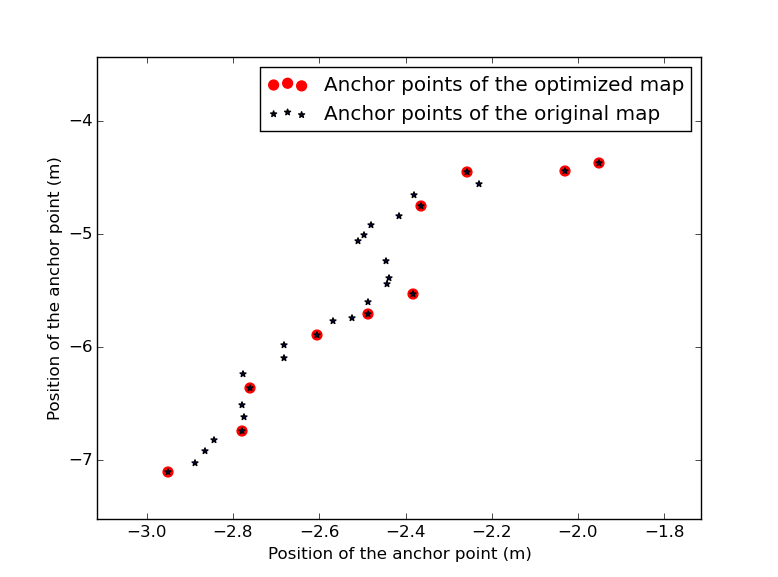
\includegraphics[scale=0.4]{map_optimization}
  \caption{Comparison of un-optimized and optimized maps}
\end{figure}

First, we implemented our topometric map optimization method conformably to section \ref{approach}.
Then, we optimized three dataset acquired during three previous \textit{teach} sessions. The
\textit{terasse} dataset is a short run paving stones on Université Laval's campus. It was a busy
summer day, and passer-by that were curious about the robot introduced noise in the point
clouds. The \textit{forest} dataset is a short run in some woodland on campus, making the environment
highly unstructured. Finally, we used \textit{hallway}, mapping an indoor hallway, as a
benchmark through the development of the algorithm. It records the robot going in a straight line.
During this \textit{teach} session the robot was tuned to record a very high number of point clouds,
so we expect the optimization algorithm to filter a lot of nodes in this case. All three datasets
were collecting using a Clearpath Husky A200 equiped with a Velodyne HDL-32e lidar sensor. The teach
sessions were executed using home-grown Teach and Repeat software.

\begin{figure}
  \centering
  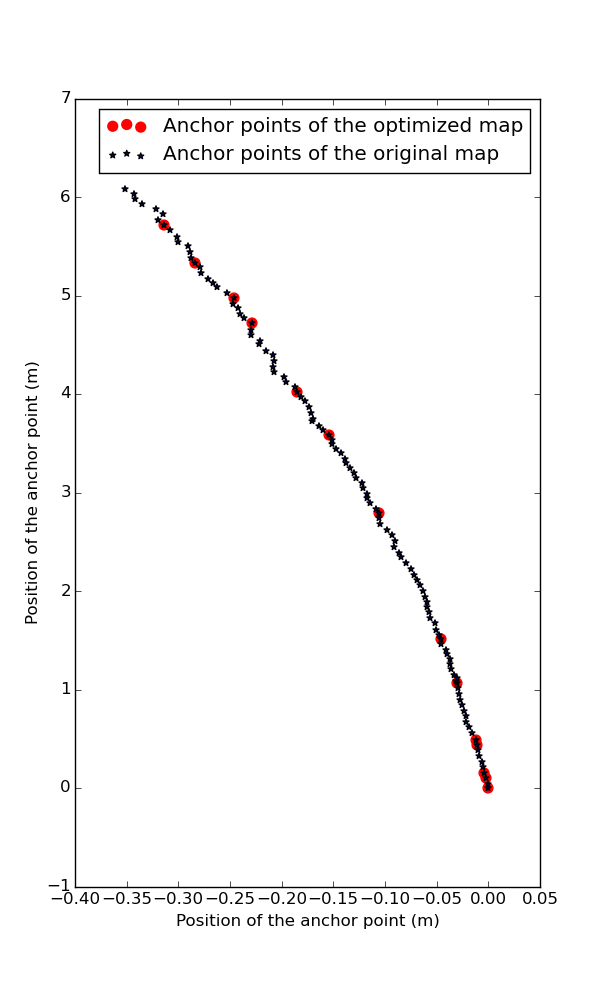
\includegraphics[scale=0.5]{hallway_optimization}
  \caption{Optimization of hallway dataset}
\end{figure}

We used parameters $a=0.4 m$, $b=0.4 m$ and $\epsilon=0.05 m$ for those optimization runs. The
optimization is indeed able to reduce the number of point clouds necessary to execute a
\textit{repeat} session. As exepected, depending on the robot trajectory some zones contain more
superfluous nodes than others. Straight lines in very static environments tend to require less
anchor points, where trajectories containing heavy rotations are less filtered out. The algorithm
tends not only to eliminate superfluous point clouds, but it also gets rid of the nodes that are
hard to localize against, for instance a point cloud containing a passer-by that is not there on the
other neighboring point clouds. For instance in the \textit{hallway} dataset, even though the
overall localization using ICP is easy, some clouds could not be used for localization at all.
Finally, the number of remaining nodes could be tuned down even more, at the cost of a lower
tolerance to error. Our algorithm thus gives the user a very direct way to control the
memory-size/ability-to-localize tradeoff. The numbers given in table
\ref{tabopti} are meant to give a general idea, but they could be very different depending on the
geometry of the environment, the parameters given by the user, and the quality of the odometry
estimates.

We noticed that in some datasets, the \textit{ICP chain} used to reconstruct the relative positions
between the nodes may be noisier than we thought, yielding unrealistic positions for sucessive
anchor points. It leaves us wondering wether we should rather rely on the odometry from the weels as
a reference transformation. A Kalmann Filter using both odometry and the results from ICP would be
optimal.

\begin{table}[h]
\centering
\begin{tabular}{|l|r|r|r|}
  \hline
Dataset & N. of nodes & N. of nodes (optimized) & \% nodes kept \\
\hline
  hallway & 117 & 14 & 12.0 \\
\hline
terasse & 304 & 186 & 61.2 \\
  \hline
forest & 62 & 41 & 66,1 \\
  \hline
\end{tabular}
\caption{The result of the optimization on different datasets}
\label{tabopti}
\end{table}


\subsection{Parameters $a$ and $b$}

We observed the effects of parameters $a$ and $b$ when optimizing the \textit{forest} dataset. As
expected, the percentage of nodes kepts after optimization grows with the tolerance ellipse. We
noticed that very small tolerance ellipses does not necessarily mean a very small amount of nodes;
that is explained by the quality of the anchor points themselves. A point cloud that has a very bas
initial position estimate, or that contains a passer-by, is always going to make the optimization
more difficult, no matter how small the tolerance ellipse is.

\begin{table}[h]
\centering
\begin{tabular}{|r|r|r|r|}
  \hline
a (m) & b (m) &  N. of nodes after optimization & \% of points kept \\
\hline
  0.2 & 0.1 & 41 & 66.1  \\
\hline
 0.4 & 0.4 & 41 & 66.1 \\
  \hline
 1.6 & 0.8 & 44 & 72.1 \\
  \hline
1.8 & 0.9 & 59 & 96.7 \\
  \hline
  2.0 & 1.0 & 61 & 100.0 \\
  \hline
\end{tabular}
\caption{The effects of parameters $a$ and $b$}
\label{tabopti}
\end{table}

\section{FUTURE WORK}

\subsection{Experiment with Husky}
In the future, we would like to validate experimentally, using a Clearpath Husky Robot, that the produced topometric map do can be used for localization.
To reach that goal, we would optimized maps acquired during the teach phase of a teach and repeat. Then, we would compare
the accuracy of the robot during the repeat phase using the optimized and unoptimized maps.

We would also want to validate experimentally the effect of the parameters $a$ and $b$ (the semi-axis of the ellipse)
on the accuracy of the map. That is, given a certain repeat run, we would like to validate that if
we optimized the map demanding a tolerance to error $x$, we are able to move the robot outside of
it's trajectory by $x$ and still be able to localize.

Finally, we would like to validate if removing nodes from the topometric map harms precision in highly unstructured environment like forests.

\subsection{Multi-objective optimization for automatic parameter selection}

To focus our efforts on fiding the minimal node subset, we made the simplication the convergence ellipse has a fixed sized.
has a fixed sized.  In other words, we manually specify the distance in $x$ and $y$ for which we
want the ICP to converge. With those parameters given, we can reduce the problem to a finding the
shortest path in a graph, as shown in section \ref{approach}.


A limitation of this approach is that, if for a given node, decreasing the size of the ellipse would
make the ICP converge on further nodes of the graph. We can see that as a tradeoff between the
precision and the number of nodes of the final map.


An improvement on the current method would be model the problem as a multi-objective optimization
problem. Given an initial ellipse size for each node of the graph, changing reducing the size of the
ellipse has a cost. The goal is to find the best tradeoff between the length of the shortest path in
the graph and the the costs of the nodes that are used by that shortest path.

\subsection{Handling rotations}

For the sake of simplicity we did not use rotations when inducing errors to the reading's
position estimate, before testing the reliability of the localization. To make the optimization
problem more difficult, while giving the user more ways garantee the reliability of the optimized
maps, we could replace $T$ the space of translations with $R \times T$ the space of rotations and
translations in function $f$. That way, the user could demand that the generated maps be tolerant to
a certain error in the orientation of the robot.

Using the whole space of rotations $R$ might be too general, as it is often useful to simplify the pose of a
ground robot begin a vector $[x, y, \theta]^t$, $\theta$ being the heading. That case could also be
handled by replacing the tolerance ellipse by an ellipsoid. The supplementary dimension would
represent the error in heading, or $\Delta \theta$.

\subsection{Reoptimization of the localizability graph}

The optimization could be taken a step further if we make one more assumption about the behavior
of the \textit{repeat} phase. So far we assumed that the repeat algorithm would work that way: when
following a trajectory passing by anchor points $a$ then $b$, the robot would use point $a$ as a
reference for localization until it is very close to $b$, and then switch reference. It would be
reasonable to have the robot behave differently and make it switch references somewhere in between
$a$ and $b$, which would make the localization easier.

This modification would allow us to make an even better optimization of the topometric maps. When
finding the shortest path in the localizability graph, we ensure that every node in the graph can be
reached by using the preceding node as a reference. This means (assuming that the ICP algorithm is
reflexive) that every second anchor point in our optimized map becomes superfluous and can be removed.

\section{Conclusion}

We introduced an offline algorithm that can greatly reduce the amount of reference points needed in
a topometric map for it to be used in a Teach and Repeat implementation. Our algorithm computes the
ability of candidate anchor points to be used as good reference when navigating a given
environment. The results of this computation are used to filter out nodes in the topometric map
until it is as small as possible to execute a \textit{repeat} run, given a demanded tolerance to
error. Our approach was tested using 3d point clouds from a lidar sensor and ICP, but is general
enough to be applied to vision-based implementations of the Teach and Repeat paradigm. Experiments
confirm that the algorithm is indeed able to optimize topometric maps, and that the user can tune
the size of the map by changing his error tolerance requirements.

\printbibliography

\end{document}
